\section{Notion de base}
\vspace{-1.75\baselineskip}
\begin{tabular}{ll}
Puissance électrique & \(P = VI = R I^2 = V^2/R\)\\
Loi d'Ohm & \(V = RI \Leftrightarrow R=V/I \)\\
Résistances en série & \(R_{\mathit{eq}}=R_1 + \dots + R_N\)\\
Résistances en parallèle & \(R_{\mathit{eq}}=\qty(\frac{1}{R_1}+\dots +\frac{1}{R_N})^{-1}\)
\end{tabular}

\subsection{Kirchhoff}
\begin{center}
\begin{tabular}{c|c}
    Loi des noeuds & Loi des mailles \\
    % $\Sigma I = 0$ & $\Sigma \Delta V =0$
    $\sum I = 0$ & $\sum \Delta V =0$
\end{tabular}
\end{center}

% \subsubsection{Étapes de résolution d'un circuit}
% \begin{enumerate}[nosep]
%     \item Assigner un courant dans chaque branche : Direction arbitraire, si le courant est négatif, alors le courant circule en sens contraire.
%     \item Écrire les équations de tous les noeuds sauf un. $(n-1)$
%     \item Écrire les équations de diverses mailles jusqu'à l'obtention de $X$ équations pour $X$ inconnues; chaque branche doit être parcourue aux moins une fois.
% \end{enumerate}
% \subsubsection{Sens du courant}


%\section{Techniques d’analyse de circuits}
% \vspace{-.5\baselineskip}
% \subsection{Transformation de source}
% \vspace{-1\baselineskip}
% Seulement possible s'il n'y a pas de source dépendante dans le circuit.
% \begin{multicols*}{2} 
% \centering
%  trim={<left> <lower> <right> <upper>}
% \includegraphics[trim={1.75in 8.375in 1.75in 1in}, clip=true,page=2,height=.85in]{fig/equiv.pdf}

% \begin{equation*}
%     I_s = \frac{V_s}{R}
% \end{equation*}
% \end{multicols*}
% \vspace{-1\baselineskip}

% % \vspace{-1\baselineskip}
% \subsubsection{Cas particulier}
% \begin{itemize}[nosep]
%     \item Résistance en $//$ avec $V_s$ peut être ignorée.
%     \item Résistance en série avec $i_s$ peut être ignorée.
% \end{itemize}


% \subsection{Équivalents Thévenin et Norton}
% \begin{equation*}
%     R_{Th}=\frac{V_{Th}}{I_{cc}}
% \end{equation*}
% Cas particulier, si le circuit n'a pas de source dépendante. 
% \begin{itemize}[nosep]
%     \item Source de tension $=$ court-circuit
%     \item Source de courant $=$ circuit ouvert
% \end{itemize}
% \subsubsection{Étapes de résolution}
% \begin{enumerate}[nosep]
%     \item Calculer la tension de Thévenin $V_{Th}$
%     \item Calculer le courant de court-circuit $I_{cc}$
%     \item Calculer la résistance de Thévenin $R_{Th}$
%     \item Re-dessiner le circuit équivalent Thévenin
% \end{enumerate}

% \subsubsection{Équivalent Norton}
% On obtient l'équivalent Norton en faisant une transformation de source de l'équivalent Thévenin.


% \subsection{Transfert maximal de puissance}
% La puissance consommée par la charge $R_L$ est: 
% %\vspace{-.5\baselineskip}
% \begin{equation*}
%     P = VI = R_L I^2 = R_L \qty(\frac{V_{Th}}{R_{Th}+R_L})^2
% \end{equation*}
% Résistance $R_L$ pour obtenir un transfert de puissance maximal
% %\vspace{-1\baselineskip}
% \begin{equation*}
%     R_L = R_{Th}
% \end{equation*}
% La puissance transférée à la charge:
% %\vspace{-.375\baselineskip}
% \begin{equation*}
%     P_{max} = \frac{V^2_{Th}}{4R_L}
% \end{equation*}
% %\vspace{-1\baselineskip}